%
% This is the LaTeX template file for lecture notes for EE 382C/EE 361C.
%
% To familiarize yourself with this template, the body contains
% some examples of its use.  Look them over.  Then you can
% run LaTeX on this file.  After you have LaTeXed this file then
% you can look over the result either by printing it out with
% dvips or using xdvi.
%
% This template is based on the template for Prof. Sinclair's CS 270.

\documentclass[twoside]{article}
\usepackage{graphicx}
\usepackage{wrapfig}
\usepackage{amsmath}
\usepackage{amssymb}
\usepackage{listings}
\setlength{\oddsidemargin}{0.25 in}
\setlength{\evensidemargin}{-0.25 in}
\setlength{\topmargin}{-0.6 in}
\setlength{\textwidth}{6.5 in}
\setlength{\textheight}{8.5 in}
\setlength{\headsep}{0.75 in}
\setlength{\parindent}{0 in}
\setlength{\parskip}{0.1 in}

%
% The following commands set up the lecnum (lecture number)
% counter and make various numbering schemes work relative
% to the lecture number.
%
\newcounter{lecnum}
\renewcommand{\thepage}{\thelecnum-\arabic{page}}
\renewcommand{\thesection}{\thelecnum.\arabic{section}}
\renewcommand{\theequation}{\thelecnum.\arabic{equation}}
\renewcommand{\thefigure}{\thelecnum.\arabic{figure}}
\renewcommand{\thetable}{\thelecnum.\arabic{table}}

%
% The following macro is used to generate the header.
%
\lstset{language=Python, numbers=left, tabsize=2, xleftmargin=5.0ex}

\newcommand{\lecture}[4]{
   \pagestyle{myheadings}
   \thispagestyle{plain}
   \newpage
   \setcounter{lecnum}{#1}
   \setcounter{page}{1}
   \noindent
   \begin{center}
   \framebox{
      \vbox{\vspace{2mm}
    \hbox to 6.28in { {\bf EE 382V: Parallel Algorithms
                        \hfill Summer 2017} }
       \vspace{4mm}
       \hbox to 6.28in { {\Large \hfill Lecture #1: #2  \hfill} }
       \vspace{2mm}
       \hbox to 6.28in { {\it Lecturer: #3 \hfill Scribe: #4} }
      \vspace{2mm}}
   }
   \end{center}
   \markboth{Lecture #1: #2}{Lecture #1: #2}
   %{\bf Disclaimer}: {\it These notes have not been subjected to the
   %usual scrutiny reserved for formal publications.  They may be distributed
   %outside this class only with the permission of the Instructor.}
   \vspace*{4mm}
}

%
% Convention for citations is authors' initials followed by the year.
% For example, to cite a paper by Leighton and Maggs you would type
% \cite{LM89}, and to cite a paper by Strassen you would type \cite{S69}.
% (To avoid bibliography problems, for now we redefine the \cite command.)
% Also commands that create a suitable format for the reference list.
\renewcommand{\cite}[1]{[#1]}
\def\beginrefs{\begin{list}%
        {[\arabic{equation}]}{\usecounter{equation}
         \setlength{\leftmargin}{2.0truecm}\setlength{\labelsep}{0.4truecm}%
         \setlength{\labelwidth}{1.6truecm}}}
\def\endrefs{\end{list}}
\def\bibentry#1{\item[\hbox{[#1]}]}

%Use this command for a figure; it puts a figure in wherever you want it.
%usage: \fig{NUMBER}{SPACE-IN-INCHES}{CAPTION}
\newcommand{\fig}[3]{
			\vspace{#2}
			\begin{center}
			Figure \thelecnum.#1:~#3
			\end{center}
	}
% Use these for theorems, lemmas, proofs, etc.
\newtheorem{theorem}{Theorem}[lecnum]
\newtheorem{lemma}[theorem]{Lemma}
\newtheorem{proposition}[theorem]{Proposition}
\newtheorem{claim}[theorem]{Claim}
\newtheorem{corollary}[theorem]{Corollary}
\newtheorem{definition}[theorem]{Definition}
\newenvironment{proof}{{\bf Proof:}}{\hfill\rule{2mm}{2mm}}

% **** IF YOU WANT TO DEFINE ADDITIONAL MACROS FOR YOURSELF, PUT THEM HERE:

\begin{document}
%FILL IN THE RIGHT INFO.
%\lecture{**LECTURE-NUMBER**}{**DATE**}{**LECTURER**}{**SCRIBE**}
\lecture{9}{June 17}{Vijay Garg}{Tiffany Tillett}
%\footnotetext{These notes are partially based on those of Nigel Mansell.}

% **** YOUR NOTES GO HERE:

% Some general latex examples and examples making use of the
% macros follow.  
%**** IN GENERAL, BE BRIEF. LONG SCRIBE NOTES, NO MATTER HOW WELL WRITTEN,
%**** ARE NEVER READ BY ANYBODY.
\section{Introduction}
During this lecture, we discussed the following popular parallel sorting algorithms: 
%During this lecture, we were exposed to the first parallel algorithm of the class (a simple array sum). We continued with this example to introduce and explore some of the fundamental concepts in parallel algorithm construction and analysis, including:
\begin{itemize}
	\item Radix Sort
	\item Merge Sort
	\item Quick Sort
\end{itemize}

This set of lecture notes will briefly re-examine the topics covered in this lecture, in the order in which they appeared during class. Note: This order is different than that of the lecture notes (lect-sort.pdf)

\section{Radix Sort}
Radix Sort is a non-comparison based sorting algorithm. It utilizes the radix $r$ to place elements into buckets based on their value. The radix is also known as the base. For example:
\begin {itemize}
	\item base 2
	\item base 8
	\item base 10
\end{itemize}

\subsection{The Deck of Cards Example}
In the case of a deck of cards, we know that there are exactly 52 cards divided into 4 suits with 13 unique cards belonging to each suit. We can create a bucket for each suit:

\begin{itemize}
	\item Spades
	\item Hearts
	\item Diamonds
	\item Clubs
\end{itemize}

Within each of these 4 buckets, we can create buckets for each of the 13 card values. Once the cards are all divided into the correct buckets, it is straightforward to put them in the correct order.

\subsection{A Numerical Illustration}
Now lets look at an example using numbers. We have an array $A = [35, 42, 71, 21, 74]$. In this case, the radix is the set of numbers ${0...9}$ and we have two digits. 

Lets look at the case where we divide based on the most significant digit $(MSD)$ first:

\begin{center}
\begin{tabular} { | c | c | c | c | c | c | c | c | c | c | c | }
\hline
radix & 0 & 1 & 2 & 3 & 4 & 5 & 6 & 7 & 8 & 9 \\
\hline
values & & & 21 & 35 & 42 & & & 71, 74 & & \\
\hline
\end{tabular}
\end{center}

We would next divide each box into ten sub-boxes and repeat for the least significant digit $(LSD)$. However, we will instead look at the case where we divide based on the $LSD$ first. 

\begin{center}
\begin{tabular} { | c | c | c | c | c | c | c | c | c | c | c | }
\hline
radix & 0 & 1 & 2 & 3 & 4 & 5 & 6 & 7 & 8 & 9 \\
\hline
values & & 71, 21 & 42 & & 74 & 35 & & & & \\
\hline
\end{tabular}
\end{center}

If we then take the elements in order, we have an array $B = [71, 21, 42, 74, 35]$. Again, we would next divide each box into ten sub-boxes and repeat for the MSD. After the second pass, we have our final sorted array $C = [21, 35, 42, 71, 74]$. \texttt{We will always be able to compute a sorted array in $d$ passes where $d$ is the number of digits.}

\subsection{The Concept of Stable Sort}
\begin{center}
$Stable Sort \equiv$ A sorting algorithm is stable if it preserves the order of entries that are equal.
\end{center}

For example, we can see that in the second pass, both $71$ and $74$ will be in buckets for $MSD = 7$. However, we must maintain the results from the first pass in order to ensure the correct final order.

\subsection{The Serial Radix Sort Algorithm}
\begin{lstlisting}
for i:= 1 to d do
	StableSort on digit i
\end{lstlisting}

This algorithm has time complexity $O(d * n)$ = $O(n)$ meaning that we iterate through all of the elements $d$ times where $d$ is the number of digits and $n$ is the size of the array.


\subsection{Parallel Radix Sort}
Lets look at the case where all numbers are binary. On the first pass, we will look at the $LSD$ (right most digit). This process will result in all elements ending in $0$ rising to the top and all elements ending in $1$ falling to the bottom. Note that we are using stable sort, so the order of the elements ending in 0 will be maintained. Similarly, the order for elements ending in one will also be maintained. We will move one place to the left and repeat the process until we have looked at all 4 digits.

\begin{center}
\begin{tabular} { | c | c | c | c | c | }
\hline
initial & after 1st pass & after 2nd pass & after 3rd pass & final \\
\hline
1011 & 0110 & 1000 & 1000 & 0000 \\
\hline
0110 & 1000 & 0000 & 0000 & 0110 \\
\hline
0111 & 0000 & 0110 & 1011 & 0111 \\
\hline
1000 & 1011 & 1011 & 0110 & 1000 \\
\hline
0000 & 0111 & 0111 & 0111 & 1011 \\
\hline
1111 & 1111 & 1111 & 1111 & 1111 \\
\hline
\end{tabular}
\end{center}

We will use a function called \texttt{compacting an array}. The steps are as follows:
\begin{lstlisting}
filter out interesting elements
make a new array with a value of 1 for the interesting elements and a value of 0 for all other elements
use scan (exclusive prefix sum) to calculate the new indices for the interesting elements
calculate the indices for the non-interesting elements
drop all elements into the new array at the correct position
\end{lstlisting}

Here is an example where we want to move all elements with the last number of 0 to the front of the array:
\begin{center}
\begin{tabular} { | c | c | c | c | c | c | c | }
\hline
A & 010 & 111 & 110 & 001 & 000 & 101 \\
\hline
match & 1 & 0 & 1 & 0 & 1 & 0 \\
\hline
scan(match) & 0 & 1 & 1 & 2 & 2 & 3 \\
\hline
B & 010 & 110 & 000 & 111 & 001 & 101 \\
\hline
\end{tabular}
\end{center}





\section{Merge Sort}
Merge Sort is a common sorting algorithm. The simple version of the algorithm is:
\begin{lstlisting}
mergesort(Left Half)
mergesort(Right Half)
merge(Left Half, Right Half)
\end{lstlisting}

The recursive calls to mergesort can be easily executed in parallel. The interesting part here is doing the merge step in parallel.

\subsection{GPU Architecture Review} 
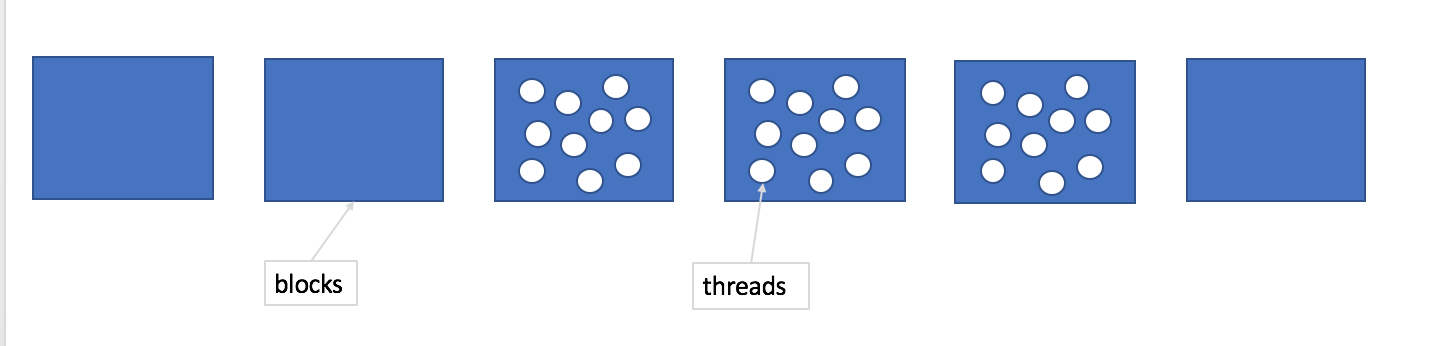
\includegraphics[scale=0.7]{img/GPU_Architecture.png}

\subsection{Maximizing Parellelism with MergeSort} 
The merge sort algorithm will divide the array in a manner similar to what is shown in the image below:
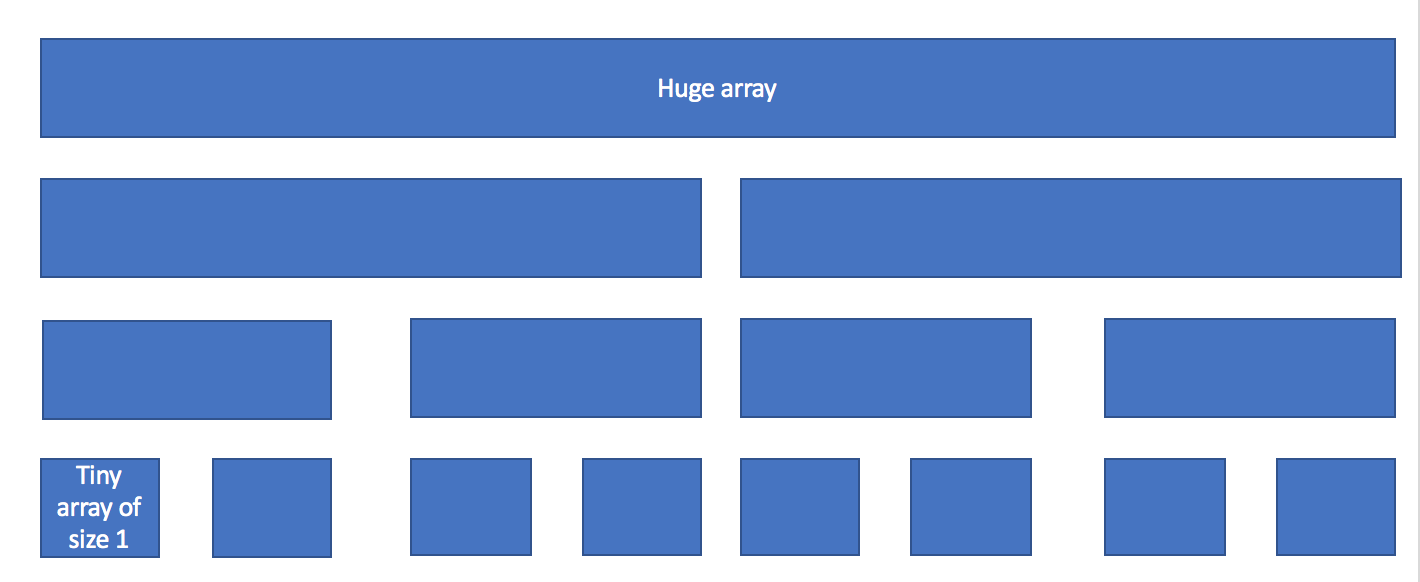
\includegraphics[scale=0.7]{img/MergeSortDivision.png}

To have maximum parallelism, we want to use as many threads as possible at any given time. We have lots of parallel merge operations happening near the bottom of the tree. We can have each thread do its own merge using the sequential algorithm since each merge is so small. As we move to the middle of the tree, we no longer have enough merge operations to make the sequential algorithm effective. Here, we will switch to the parallel merge algorithm that was discussed in a previous lecture (lect-merge.pdf). Near the top of the tree, we have only a few large merges. Here, we will divide each merge into a lot of merge tasks to create parallelism. The idea here is that we choose our merge algorithm based on the size of the arrays that we are merging.

An example of this on the GPU would be:

Stage 1: Within a block, we can use many threads to compute the small merge threads.

Stage 2: At a certain point, each block will only have two sections to merge (one merge task). This is when we switch to the parallel merge algorithm.

Stage 3: Once each block has completed its merging, we now need to merge the results from each block to get the final result. Here is where we use the idea of splitters to break each merge task into multiple merge tasks so that each merge task can be assigned to a different block.

Using parallel merge, we have:

$T(n) = T(n/2) + O(log n)$

$T(1) = 1$

$T(n) = O(log^2 n)$

\subsection{Merge Sort in $log n$ time?}
There is a complicated algorithm called Cole's Algorithm which can do sort in $O(log n)$ time. However, this algorithm comes with a lot of overhead and is not used in practice.


\section{QuickSort}
The concept of QuickSort is as follows:
\begin{lstlisting}
choose a pivot element
partition the array
	all elements smaller than the pivot will be to the left of the pivot
	all elements larger than the pivot will be to the right of the pivot
	the pivot will be in its final sorted position
quicksort(left)
quicksort(right)
\end{lstlisting}

The entire algorithm will take $O(n^2)$ time in the worst case and $O(n logn)$ time in the average case.

Let's look at a hypercube example.

Assume that we have $p$ processors and each node has a chunk of the array where each chunk is of size $n/p$.
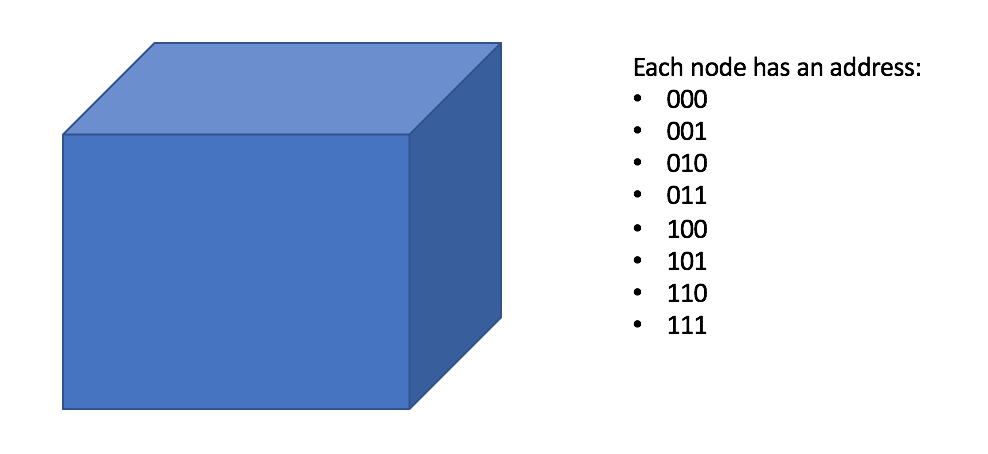
\includegraphics[scale=0.7]{img/HyperCube.png}

\subsection{QuickSort Algorithm 1: Parallel QuickSort}
\begin{lstlisting}
Some processor chooses a pivot value x
That processor broadcasts x to all processors
Each processor will partition their portion into two parts ( <= x, > x)
Assign each processor a partner
Each partner will exchange their unneeded portion with their partner.
	If I am 000, I will send values > x to 100
	If I am 100, I will send values <= x to 000
proceed recursively until the array is sorted
\end{lstlisting}


\subsection{QuickSort Algorithm 2: HyperQuickSort}
\begin{lstlisting}
Each processor will sort its own portion
Processor0 chooses the median as the pivot
Processor0 broadcasts to all processors
Proceed as above except we exploit the fact that all arrays are sorted.
\end{lstlisting}


\end{document}





Contact GitHub API Training Shop Blog About
� 2017 GitHub, Inc. Terms Privacy Security Status Help